\section{Magnetic field}

\begin{Exercise}[difficulty=1]
Find direction and value of magnetic field H produced by current I in the point P. 
\begin{center}
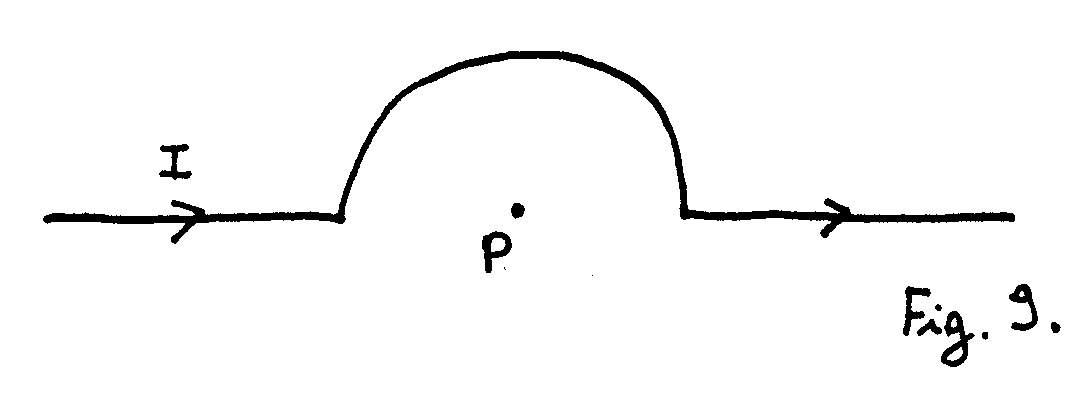
\includegraphics[width=0.4\textwidth]{img/fig_m1.png} 
\end{center}
\end{Exercise}

\begin{Exercise}[difficulty=3]
Using Ampere's Circular Law describe distribution of magnetic field vector inside, and outside coaxial cable.
\begin{center}
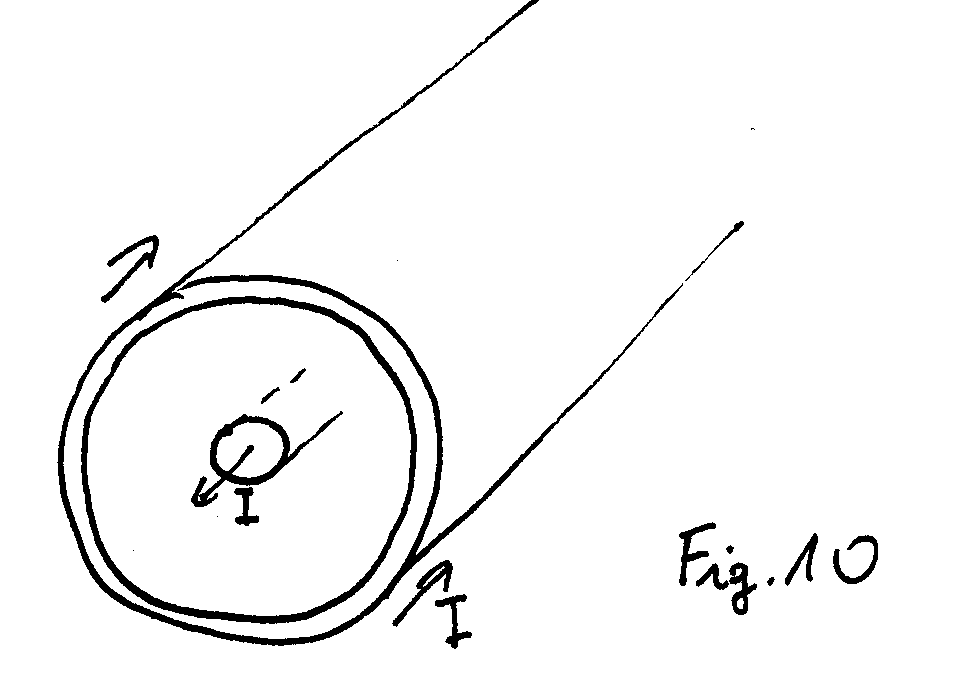
\includegraphics[width=0.4\textwidth]{img/fig_m2.png} 
\end{center}
\end{Exercise}

\begin{Exercise}[difficulty=2]
Two long, parallel cables with the same values but opposite directions of DC current are producing magnetic field around them. Find H distribution on the plane defined by two cables. 
\begin{center}
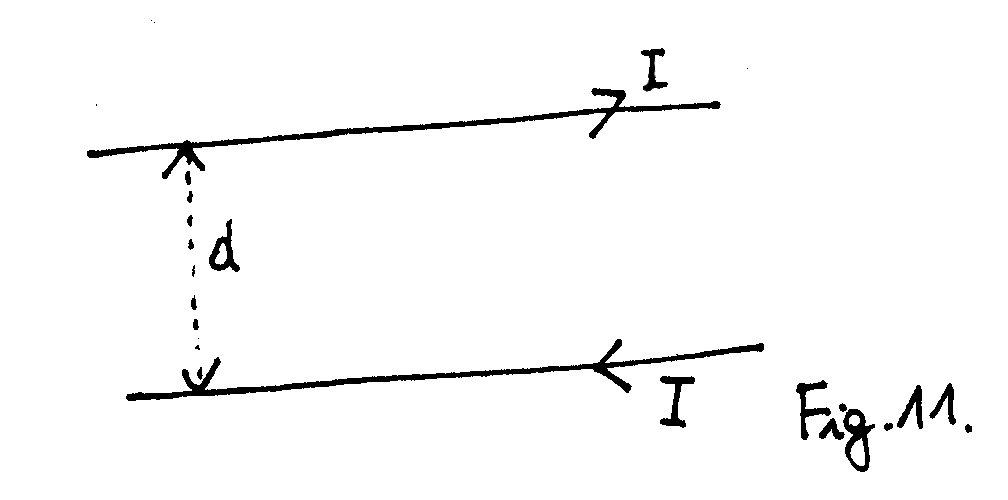
\includegraphics[width=0.4\textwidth]{img/fig_m3.png} 
\end{center}
\end{Exercise}
